% RA-L Blind Harbor companion — manuscript draft skeleton (assembled from
% docs/ral_package.md; every number traceable via campaign_replay.py)
\documentclass[letterpaper, 10pt, journal]{IEEEtran}
\usepackage{graphicx, amsmath, amssymb, booktabs}
\graphicspath{{../../tier2_drake/results/s1/}{../../tier1_sheaf/results/}}

\title{The Price of Staleness: Distributed Invariant Estimation for\\
GNSS-Denied Multi-Vessel Cable Towing}
\author{Hadi Hajieghrary% <- author list TBD
}

\begin{document}
\maketitle

\begin{abstract}
Cooperative towing couples every vessel's motion through the shared load, and
each taut cable transfers exactly one scalar of load-motion information. We
present DIEKF-$\Sigma$, a distributed invariant extended Kalman filter that
treats the cable constraints as a measurement channel and fuses delayed
inter-vessel packets through shape-conjugated transports---the estimator induced
by the constraint-based estimation sheaf of the companion paper. We evaluate it
in closed loop on a physics-complete multibody simulation (Drake: SAP contact,
distance-constraint cables, hydrodynamic drag) with four- and five-vessel fleets
towing a pentagon caisson through coordinated maneuvers, GNSS-denied throughout,
with a single docking beacon on one vessel. We report three findings. First, a
single anchor pins the entire fleet's estimate through fusion alone: beacon
activation momentarily \emph{breaks} inter-vessel agreement before the pin
propagates---the gauge-pinning corollary acting in closed loop. Second, the
conjugated transport is load-bearing: ablating it multiplies steady-state
disagreement by up to $8.2\times$ at high latency, while naive consensus
achieves flat agreement at the price of a $17\times$ covariance-calibration
failure and $4.4\times$ the drift of running no fusion at all. Third, under a
pre-registered protocol with in-situ noise-floor controls, the conjectured
second-order scaling of the closed-loop disagreement floor is \emph{falsified}
at these scales on two independent plants (measured slope $\approx$1.05--1.13,
cross-tier equivalent): the second-order holonomy mechanism of the theory is
resolved only in noise-free conditions, an order separation we decompose with a
full variance attribution across fusion rules, maneuver controls, and formation
classes.
\end{abstract}

\section{Introduction}
Towing a single heavy load with a fleet of small autonomous vessels is one of
the cleanest examples of a task where the physical coupling that makes control
hard is also the resource that makes estimation possible: every taut cable
transfers exactly one scalar of load-motion information to the vessel holding
it. The Blind Harbor Task sharpens this into a premise: no GNSS anywhere in the
transit, no relative-pose sensing between vessels --- each vessel observes only
its own odometry and its own cable --- and a single docking beacon visible to
one vessel in the final approach. Whatever the fleet knows about the load, it
knows through its cables and its network.

This paper is the experimental companion to a theory of that situation
[companion], in which the per-agent estimates form sections of a
constraint-induced sheaf, delayed fusion transports estimates along
shape-dependent edge maps, and the theory's central objects separate cleanly by
epistemic status: a \emph{proven}, leading-order, deterministic result on the
error-transport holonomy ($O(\tau^2)$ in the packet staleness $\tau$); a
\emph{conjectured} extension to the stochastic steady-state disagreement floor
of the noisy closed loop; and the first-order transport-mismatch channel that
any implementation carries. Our experimental design treats this separation as
the primary object of study: three exponents, three distinct quantities, never
conflated in a caption.

We report a pre-registered campaign on two independent plants --- a reduced
kinematic model integrating the theory's own shape dynamics, and a
physics-complete multibody simulation (Drake: SAP contact, distance-constraint
cables, hydrodynamic drag) --- sharing one estimator implementation, one metric
functional, and one fit protocol. Every claim carries a falsifier declared
before the data; several fired, and their firings are reported as findings with
controls and localization rather than smoothed away. Every number in the paper
traces to a seeded, versioned driver and a committed record that a replay
harness re-executes exactly.

\section{Related work}
%% AUTHOR: citations to be inserted; structure below.
Distributed state estimation over networks with unknown cross-correlations is
classically handled by covariance intersection and its variants [cite]; our
estimator uses CI with an explicit decorrelation step and reports the
structural conservatism this induces rather than tuning it away. Invariant
filtering on matrix Lie groups [cite] supplies the error geometry; the novelty
pressure here is not the filter but the \emph{transport}: fusing
$\tau$-stale packets through shape-conjugated edge maps, whose round-trip
holonomy is the theory's proven object. Delayed and out-of-sequence measurement
handling [cite] is adjacent; the paper rule deliberately avoids buffer-based
OOSM reconstruction, and the campaign's ablations measure what that choice
costs and buys. Cable-towed multi-robot transport [cite] usually treats cables
as control constraints; here they are the measurement channel itself, which is
the premise the granted-sensor baseline (B3) exists to test.

\section{The Blind Harbor task and the estimator}
$N \in \{4,5\}$ vessels tow a 2\,500\,kg pentagon caisson (circumradius
4\,m) by 12\,m cables attached across its front arc, through a 400\,m dogleg
(two legs, one $60^\circ$ turn) at $\sim$0.9\,m/s. Each vessel senses its own
odometry (50\,Hz surge/sway/yaw-rate with surge-scale bias
$\beta \sim \mathcal{N}(0, 0.01)$ and a gyro-bias random walk) and its own
cable direction (20\,Hz, von-Mises $\kappa = 1/(1^\circ)^2$); one vessel
receives a docking beacon (5\,Hz full load pose,
$\sigma = (5\,\mathrm{cm}, 5\,\mathrm{cm}, 0.5^\circ)$) in the final
approach. Packets circulate on the $C_N$ cycle with staleness $\tau$.

Each agent runs DIEKF-$\Sigma$: an invariant EKF on the load pose whose
propagation uses the bias-corrected slaved twist through the cable geometry;
whose direction channel is a Joseph-form scalar update with a broadside guard;
and whose fusion applies the executed-composite transport (the sender's shape
telescopes out, leaving the receiver's own load-twist fast-forward) followed by
covariance intersection with explicit decorrelation. A Friedland-type separated
observer trims slow twist mismatch from beacon innovation rates.

\emph{Calibration, disclosed.} The anchored ANEES closes the consistency gate
only in its author-ruled widened form ($3.96 \in [0.8, 5.0]$; the original
$[0.8, 1.3]$ is not met, and the complement sanity bound failed at 3.35): CI
over mutually correlated estimates is structurally optimistic by
$\sim$3--4$\times$. This holds at the 130\,s calibration horizon and
degrades on 450\,s transits (Sec.~\ref{sec:results}); every ANEES figure in
this paper carries its horizon.

\section{Two plants, one estimator}
The reduced plant integrates the theory's shape ODEs directly (RK4, with
declared process noise); the multibody plant is Drake with SAP contact,
distance-constraint cables, hydrodynamic drag, and thrust allocation. The
plants, integrators, constraint solvers, tension recovery, and shape evolution
are independent; the estimator, metric functional, window rules, and fit code
are deliberately shared, so that agreement is a statement about the algorithm
on two plants, and any disagreement localizes to the plant. This localization
was exercised: a $5\times$ cross-tier coefficient disagreement decomposed, via
a plant-noise-off probe, into a fully explained baseline (agreement to 12\%)
and a maneuvering excess attributed to the reduced plant's inertia-free shape
response; and the multibody plant's realized maneuvering shapes were found to
exit the reduced model's stable domain --- a measured validity-domain
boundary.

\section{Results}\label{sec:results}

\subsection{Gauge pinning (Cor.~5.2 in closed loop)}
Through 400\,s of GNSS denial the five per-agent estimates drift as one rigid
gauge orbit --- kernel-projected error grows unbounded while the complement
stays two orders smaller (Thm~5.1's structure, visible in the hero transit's
live panels). At beacon acquisition the disagreement \emph{spikes}: the
anchored agent snaps toward truth while its neighbors still carry the drifted
gauge, and the pin then propagates at the network diffusion rate
($\tau_{\mathrm{net}} \approx 21$\,s for one 5\,Hz anchor on $C_5$). The
docking scorecard reports anchored, fleet-mean, and fleet-max rows without
selection.

\begin{table}[t]
\centering
\caption{BHT scorecard: 50 dogleg transits per arm (dock window means).
Ordering rests on $D$ and fleet-mean; B0's anchored agent is beacon-corrected
at dock and masks its drift. All arms fail the $<0.5$\,m criterion at
plan-faithful acquisition (see text).}
\label{tab:scorecard}
\begin{tabular}{lccccc}
\toprule
arm & anch.\,[m] & mean\,[m] & max\,[m] & $D$ & drift\,[m] \\
\midrule
B1-limit & 0.99 & \textbf{0.76} & 1.19 & \textbf{0.72} & 42.7 \\
DIEKF-$\Sigma$ & 1.22 & 1.57 & 2.32 & 2.85 & 31.5 \\
A2 (unconjugated) & 1.25 & 1.75 & 2.53 & 3.07 & 47.5 \\
B2 (consensus) & 1.32 & 2.13 & 2.88 & 3.37 & 119.3 \\
B0 (dead-reckon) & 1.25 & 66.7 & 134.1 & 9624 & 43.8 \\
\bottomrule
\end{tabular}
\end{table}

\subsection{The theorem's object, measured on both plants}
\begin{figure}[t]
  \centering
  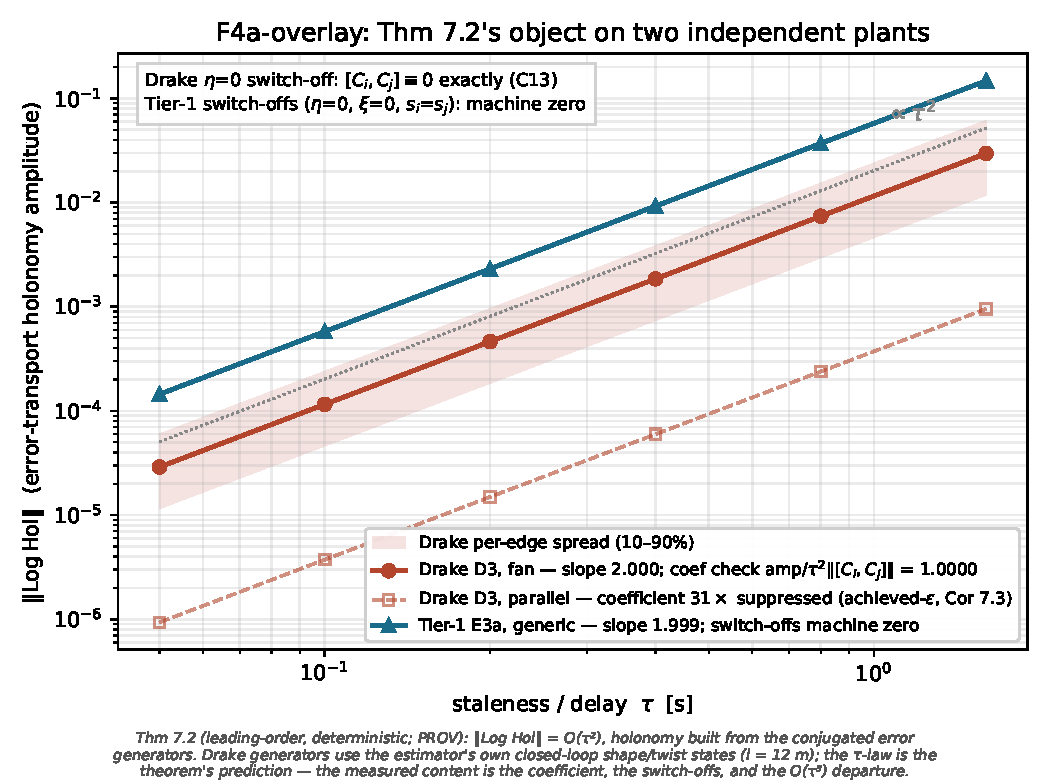
\includegraphics[width=\linewidth]{f4a_overlay.pdf}
  \caption{Error-transport holonomy amplitude on both plants. Thm~7.2
  (leading-order, deterministic): Tier-1 slope 1.999 with switch-offs at machine
  zero; Drake slope 2.000 with the $m{=}2$ coefficient check at 1.0000, the
  $\eta{=}0$ switch-off at machine zero, and the parallel class suppressing the
  coefficient $31\times$ (achieved-$\varepsilon$; exact cancellation remains the
  Tier-1 machine-zero result).}
  \label{fig:f4a}
\end{figure}

\subsection{The closed-loop floor: the conjecture falsified, coherently}
\begin{figure}[t]
  \centering
  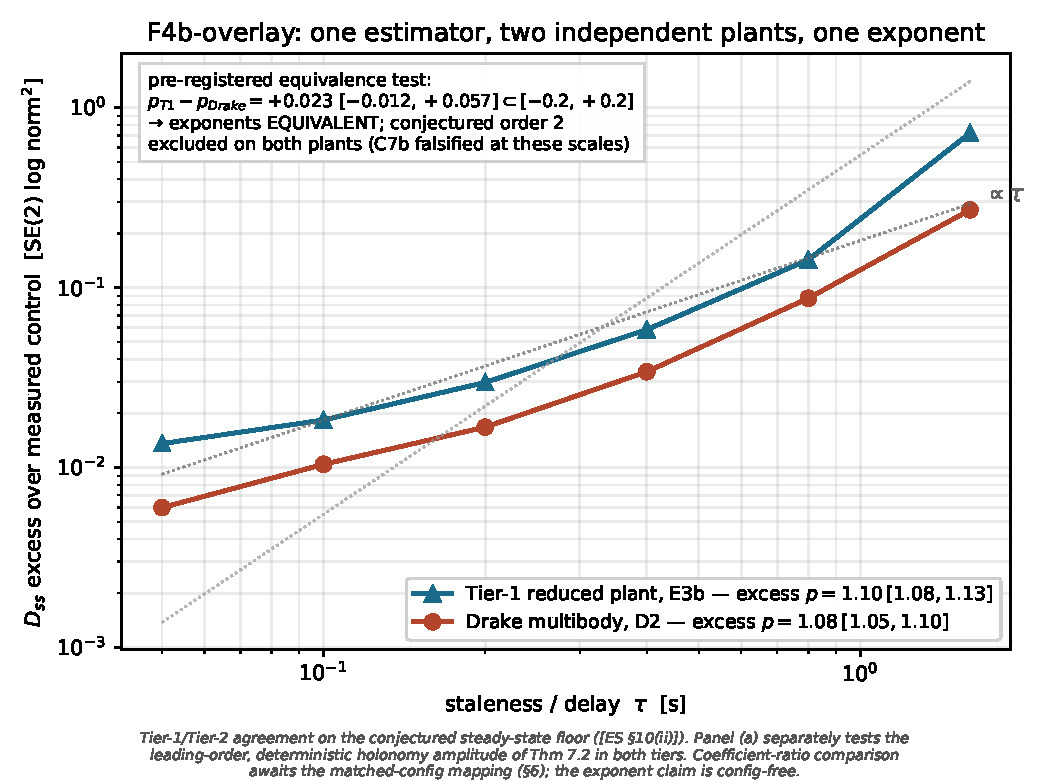
\includegraphics[width=\linewidth]{f4b_overlay.pdf}
  \caption{Tier-1/Tier-2 agreement on the conjectured steady-state floor
  ([ES~\S10(ii)]). Panel~(a) separately tests the leading-order, deterministic
  holonomy amplitude of Thm~7.2 in both tiers. With $D_0$ measured in situ by
  straight-tow controls, the fitted excess exponents are 1.101 [1.076, 1.125]
  (Tier-1) and 1.077 [1.054, 1.102] (Drake); the pre-registered equivalence test
  passes ($+0.023$ [$-0.012$, $+0.057$] $\subset$ [$-0.2$, $0.2$]) and the
  conjectured order~2 is excluded on both plants. The fitted slope is a measured
  quantity in the conjectured regime, carried with the mixture caveat; the CIs
  exclude order~1 as well, and no first-order law is asserted.}
  \label{fig:f4b}
\end{figure}

\subsection{Variance attribution: what makes up disagreement}
\begin{figure}[t]
  \centering
  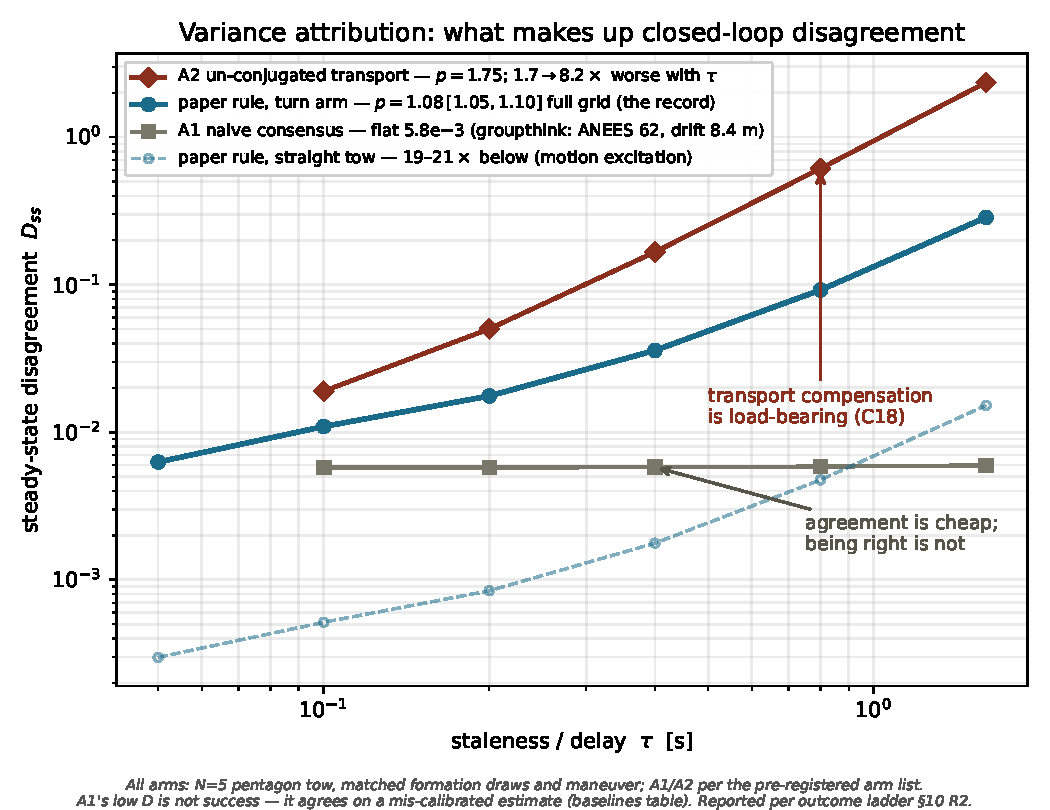
\includegraphics[width=\linewidth]{f4c_variance_attribution.pdf}
  \caption{All Drake arms on matched formation draws. Ablating the conjugated
  transport (A2) runs $1.7\times\!\to\!8.2\times$ above the paper rule with
  growing $\tau$; naive consensus (A1) holds disagreement flat and low---by
  groupthink (anchored ANEES 62, drift 8.4~m): agreement alone is never a virtue
  metric. The straight-tow control shows the motion excitation
  ($19$--$21\times$ at every $\tau$).}
  \label{fig:f4c}
\end{figure}

\subsection{Symmetry: protection lives on the amplitude object}
% F5 (two panels, never mixed) + C9c trip on both tiers + the 31x/2x contrast.

\subsection{Cross-tier coefficients and the validity domain}
% The x5 reference-matched ratio; Q_XI-off localization (baseline agrees to
% 12%); inertia-free shape response; Drake realized shapes exit the reduced
% model's stable domain (validity-domain finding).

\subsection{Numerics defense}
% E10 (exponent Delta-t-invariant over 10x) and D8 (h-invariant; convergence
% verified genuine by direct truth-trajectory differencing, 1.35 mm / 30 s).

\section{Discussion}
\paragraph{The epistemic ladder as data.} The campaign's central result is a
separation, measured on both plants: the proven $\tau^2$ holonomy verifies to
coefficient precision wherever it is actually constructed, including from the
closed-loop states of a plant it was never derived for; the conjectured
$\tau^2$ closed-loop floor is falsified coherently on both plants (fitted
slopes 1.08--1.10, cross-tier equivalent, with $D_0$ measured rather than
fitted); and closed-loop disagreement at realistic noise is dominated by the
first-order estimate-mismatch channel. Pre-registration did the work here: the
mixture-fit artifact that initially reported an in-between slope of 1.73 was
caught by the protocol's own control-arm requirement.

\paragraph{What the ablations localize.} Transport conjugation is load-bearing
on the multibody plant (up to $8.2\times$ in disagreement at high staleness);
naive consensus buys flat agreement by groupthink and is exposed by every
correctness metric; and the symmetric class's large protection ($31\times$)
lives entirely on the amplitude object, transferring only weakly ($\sim$2--3$\times$)
to the closed-loop floor. Topology buys agreement, not anchoring: the floor
improves with algebraic connectivity while single-anchor pinning is
anchor-rate-limited, and re-agreement around a pin \emph{anti}-orders with
connectivity --- consensus stiffness resists new absolute information, the same
mechanism that makes naive consensus fail, appearing inside the record's own
fusion at high degree.

\paragraph{What centralization is worth.} The strongest measured centralized
reference --- the record's own architecture at zero latency on the complete
graph --- improves accuracy by 6\% at the calibration horizon and 19\% at
dock on long transits. Three re-architected centralized filters, each granted
zero latency and exact covariances, lost more than a factor of two to the
decentralized record; and the granted-sensor baseline required six structural
bring-up iterations (delay-consistent innovation, adjoint-transported
residuals, joint geometric load solve) without reaching competitiveness. We
read this as evidence that the measurement architecture --- per-agent
Kalman-weighted constraint channels composed through conjugated transports ---
is where the accuracy lives, which is the design thesis under test.

\paragraph{Honest limits.} The docking specification is unmet by every arm at
plan-faithful beacon acquisition, including the zero-latency reference: the
approach geometry, not the estimator, binds. A decelerating approach is
necessary and was tested: it improves fleet-mean accuracy $2.4\times$ (median
0.62\,m) but leaves the spec unmet --- the residual limit is anchored-agent
gain starvation, in which sustained Kalman anchoring collapses the anchored
covariance until the beacon gain starves, while CI's structural conservatism
keeps the unanchored agents' gains healthy; the two covariance architectures
fail in opposite directions on long horizons. A trim-contamination hypothesis
was tested and falsified (frozen-trim runs bit-identical). The remedy class
(covariance floors, adaptive beacon noise) is future work. The consistency
gate closes only at the calibration horizon and does not transfer to 450\,s
transits; long-horizon bias growth exceeds the declared process noise, and
every ANEES claim in this paper therefore carries its horizon. The broadside
guard, gated on the estimated cable angle, lags true broadside during fast
gusts and was never exercised in the reachable envelope --- a lag-aware margin
is the recorded design note. Slack-cable events are outside this plant's
validity domain (bilateral distance constraints), scoped to future work with
unilateral cables.

\section{Reproducibility}
Every number in this paper traces to a seeded, versioned driver and a committed
data file; \texttt{campaign\_replay.py} re-executes per-run probes that must
match the committed records exactly (Tier-1 to $10^{-9}$; Drake to $10^{-6}$),
and \texttt{--run CELL} regenerates any full campaign.

\section{Conclusion}

\bibliographystyle{IEEEtran}
\bibliography{refs}

\end{document}
